
\chapter{Canonical Ensemble}

Often we are not interested in single particles, but rather in macroscopic quantities of particular systems. An example is the simulation of some cooling device for a building or the heating and the heat dependent drag on the surfaces in some fluids (e.g. planes, car profiles, ...). In all these cases one is only interested in local quantities such as temperature, pressure, chemical composition, density etc. In such situations only \textbf{macroscopic effects} are of interest and to simulate them  techniques that are strongly related to MD can be used very effectively. In this section, some of them are presented. Particular attention is paid to the \textbf{Nos\'e-Hoover thermostat} and the \textbf{Parrinello-Rahman barostat}. For further readings,  \citet{sim_liq} is recommended.

\vspace{0.6cm}
Typically, experiments are conducted at \textbf{constant temperature} (e.g. room temperature) and not at constant energy. This is a common situation, since systems are usually able to exchange energy with the surrounding. We will therefore couple our system to a \textbf{heat bath} to realize this situation. There are various options to do this:

\begin{itemize}
\item \textbf{Rescaling of velocities}
\item \textbf{Introduce constraints (Hoover)}
\item \textbf{Thermostat (Nos\'e-Hoover)}
\item \textbf{Stochastic method (Anderson)}
\end{itemize}

\vspace{.8cm}

\subsubsection*{Temperature and Instantaneous Temperature:}
Before starting the discussion of the methods, we will define what is meant when we speak about temperature. In a theoretical ansatz, we can start from the equipartition theorem
\begin{equation}
\avkl{p_i^{\kl{\alpha}} \pder{\mathcal{H}}{p_i^{\kl{\alpha}}}} = \avkl{q_i^{\kl{\alpha}} \pder{\mathcal{H}}{q_i^{\kl{\alpha}}}} = kT
\label{eq:equipartition}
\end{equation}

\noindent
and the classical Hamiltonian that describes the energy of the system:
\begin{equation}
\mathcal{H}=
\sum_{i=1}^{N}{\frac{\vec{p}^{\,2}_i}{2m_i}+\mathcal{V}\kl{\vec{x}_1,...,\vec{x}_N}}
\label{eq:hamilton3}
\end{equation}

Combining \eqref{eq:equipartition} and \eqref{eq:hamilton3} one obtains

\begin{equation}
3 kT = \avkl{\vec{p}_i \pder{\mathcal{H}}{\vec{p}_i}} =
\sum_{\alpha}{p_i^{\kl{\alpha}}\frac{\vec{p}^{\,2}_i}{2m_i}} = 
2 \frac{1}{2 m_i} \avkl{\vec{p}^{\,2}_i} = 2 \avkl{E_{kin,i}}
\end{equation}


and we define  the instantaneous temperature $\mathcal{T}$ as:
\begin{equation}
\mathcal{T}\equiv \frac{2}{k\kl{3N-3}} \sum_{i=1}^N {\frac{\vec{p}_i^{\,2}}{2m_i}}.
\end{equation}

The factor 3 can be thought as for the overall translation of the system (in 3D), which does not account for the temperature of the system.



\section{Velocity rescaling}


Let us now simulate a system at given fixed temperature $T$. In classical mechanics, we know that temperature corresponds to a certain kinetic energy, so we should be able to control the temperature by changing the velocities of the particles. If the system rolls away from the desired temperature we simply rescale the velocities by a factor $\alpha$:
\begin{equation}
\vec{v}_i \rightarrow \alpha \vec{v}_i.
\end{equation}
The measured temperature scales proportionally to the squared velocities, thus 
\begin{equation}
\mathcal{T} \rightarrow \alpha^2 \mathcal{T},
\end{equation}
which means that to stay at the desired Temperature $T$ we must use
\begin{equation}
\alpha = \sqrt{\frac{T}{ \mathcal{T}}}
\end{equation}
This method might seems to be very effective. However, the price that one pays for this alteration is that the physics of the system is not respected and there are serious consequences. An example is the velocity distribution that does not recover the expected canonical velocity distribution (the Boltzmann distribution). This problem can be softened by some relaxation time 
\begin{equation}
\alpha = \sqrt{1 + \frac{\Delta t}{t_T}\kl{\frac{T}{\mathcal{T}}-1}}
\label{eq:relaxation}
\end{equation} 
but this does not solve the problem. In fact, this method can be used safely only to initialize a configuration at a given temperature, but it should not be used to simulate a heath bath.

\section{Constraint method}

A more subtle way of influencing the system is adding a friction term to the classical equation of motion:
\begin{equation}
\dot{\vec{p}} = f_i - \xi \vec{p}_i, 
\label{eq:fric_term}
\end{equation}
where $\vec{p}_i = m_i \dot{\vec{x}}_i$. In Hoover's original proposal the condition for constant temperature was enforced via Lagrange multipliers: the condition of constant temperature
\begin{equation*}
0=\dot{\mathcal{T}} \propto \dder{\sum_{i=1}^N {\vec{p}_i^2}}{t} \propto \sum_{i=1}^N {\dot{\vec{p}}_i\vec{p}_i} =  \sum_{i=1}^N { \kl{f_i-\xi\vec{p}_i}  \vec{p}_i} 
\end{equation*}
implies for the Lagrange multiplier $\xi$:
\begin{equation}
\xi = \frac  {  \sum_{i=1}^N {f_i\vec{p}_i}   }  {   \sum_{i=1}^N { \abs{\vec{p}_i}^2  }    } 
\end{equation}






Considering the Taylor expansion of the relaxation of the constraint method \eqref{eq:relaxation}, Berendsen proposed


\begin{equation}
\xi = \gamma \kl{1-\frac{T}{\mathcal{T}}}
\end{equation}

which can be seen as a Taylor expansion of \eqref{eq:relaxation}, for small $\Delta t$ and $\mathcal{T}-T$ giving
\begin{equation*}
\xi = \frac{1}{2t_T\mathcal{T}} \kl{\mathcal{T}-T} \Rightarrow \gamma \approx \frac{1}{2t_T}.
\end{equation*}
As the velocity rescaling method, this method conserves temperature but it does not recover the correct velocity distribution. As \eqref{eq:fric_term}, it is also a modification of the physics of the system, and one should not expect results that are realistic in all their aspects.





\section{Nos\`e-Hoover thermostat}

This method is the only one that actually respects the physics of a system connected to a heath bath. Suichi Nos\'e introduced a new degree of freedom $s$ that describes the heath bath (\citet{nose} and \citet{nose2}). It is connected to a potential energy
\begin{equation}
\mathcal{V}\kl{s} = \kl{3N+1}kT\ln{s}
\end{equation}
and  a kinetic energy
\begin{equation}
K\kl{s} = \frac{1}{2} Q \dot{s}^2
\end{equation}
Now one can work with the conservation of the energy of the whole system (particles and heat bath) allowing energy to be exchanged between the bath and the particles to mantain the temperature constant. Until now, we always used an explicit integration method for solving the equations. We did this using a fixed time step $\Delta t$. The new degree rescales the time step:

\begin{equation}
\text{dt}'=s\text{dt}
\end{equation}

With the time rescaled, the whole Hamiltonian changes. One of the consequences is that the velocities change, and they have to be rescaled too:

\begin{equation*}
\vec{v}_i\,' = \frac{\text{d}\vec{x}_i}{\text{dt'}} = \frac{\text{d}\vec{x}_i}{\text{dt}} \frac{\text{dt}}{\text{dt'}} = \frac{\vec{v}_i}{s},
\end{equation*}

thus the energy is also changed. The new Hamiltonian can be rewritten as:

\begin{equation}
\mathcal{H} = \sum^N_{i=1}{ \frac{\vec{p}^{\,\prime 2}_i}{2m_is^2} } + \frac{1}{2}Q \dot{s}^2 + \mathcal{V}\kl{\vec{x}_1,...,\vec{x}_N} + \mathcal{V}\kl{s}.
\end{equation}
The scaling of time affects all the properties of the system, included the momenta of the particles. Once the Hamiltonian is known, we can calculate all the remaining parameters of the system in which we are interested:

\begin{itemize} 
\item momentum and force: 
$$\vec{p}_i^{\,\prime}= m_is^2\dot{\vec{x}}_i$$ 
\begin{align*}
\vec{f}_i &= \frac{\text{d}\vec{p}_i^{\,\prime}}{\text{dt}'} =-\pder{\mathcal{H}}{\vec{x}_i'}=-\nabla_{\vec{x}_i}\mathcal{V}\kl{\vec{x}_1,...,\vec{x}_N} \\
&= 2m_i s \dot{s}\dot{\vec{x}}_i + m_is^2\ddot{\vec{x}}_i
\end{align*} 
$$\frac{\text{d}\vec{p}_s}{\text{dt}'} =-\pder{\mathcal{H}}{s} = \frac{1}{s}\kl{    \sum^N_{i=1}{ \frac{\vec{p}_i^{\,\prime 2}}{2m_is^2} }  -  \kl{3N+1}kT   } $$   
\item velocities:  
$$\frac{\text{d}\vec{x}_i}{\text{dt}'} = \pder{\mathcal{H}}{\vec{p}_i^{\,\prime}}=\frac{\vec{p}_i^{\,\prime}}{m_i s^2}$$ 
$$ \frac{\text{d}s}{\text{dt}'} = \pder{\mathcal{H}}{\vec{p}_s}=\frac{p_s}{\mathcal{Q}}   $$
\end{itemize}


The  equations of motion of the particles and the heat bath can be easily derived from the Euler-Lagrange equations:

\begin{equation}
m_is^2 \ddot{\vec{x}}_i = \vec{f}_i - 2 m_i \dot{s} s \dot{\vec{x}}_i \hspace{.5cm} \text{with } i\in\mkl{1,...,N}
\label{eq:nos_motion1}
\end{equation}

\begin{equation}
Q \ddot{\vec{s}} = \sum^N_{i=1}{ m_is\dot{\vec{x}}_i^2 }  -  \frac{1}{s}\kl{3N+1}kT   
\label{eq:nos_motion2}
\end{equation}

In this case the system conserves energy, and the velocities are distributed as expected. Note that the equations \eqref{eq:nos_motion1} and \eqref{eq:nos_motion2} are coupled. This reflects the fact that the two systems are not isolated and can exchange energy in form of temperature. Clearly, one is more interested in the real time equations than in the equations in rescaled time. In order to obtain this, one has to rescale the virtual time into the real time: $\Delta t = \frac{\Delta t}{s}$:

\begin{itemize}
\item velocities:  $$\frac{\text{d}\vec{x}_i}{\text{dt}} = s \frac{\text{d}\vec{x}_i}{\text{dt}x} =\frac{\vec{p}_i^{\,\prime}}{m_is} = \frac{\vec{p}_i^{\,\prime}}{m_i}  $$  $$\frac{\text{d}s}{\text{dt}} = s \frac{\text{d}s}{\text{dt}'} =s \frac{\vec{p}_s}{Q}  $$
\item forces:  $$\frac{\text{d}\vec{p}_i}{\text{dt}} =s \frac{\text{d}}{\text{dt}'}\kl{\frac{\vec{p}_i'}{s}} = \frac{\text{d}\vec{p}_i^{\,\prime}}{\text{dt}'} - \frac{1}{s} \frac{\text{d}s}{\text{dt}'}\vec{p}_i^{\,\prime}   =  \vec{f}_i -  \frac{1}{s} \frac{\text{d}s}{\text{dt}}\vec{p}_i$$   $$\frac{\text{d}\vec{p}_s}{\text{dt}} =s \frac{\text{d}p_s}{\text{dt}'} =\sum^N_{i=1}{\frac{\vec{p}_i^{\,2}}{m_i}} - \kl{3N+1}kT $$
\end{itemize}

The equations \eqref{eq:nos_motion1} and \eqref{eq:nos_motion1} can also be expressed in the form of a system with viscous friction. Defining $\xi\equiv \der{ln\kl{s}}{t} = \frac{\dot{s}}{s}$, yields


\begin{equation}
\ddot{\vec{x}}_i =\frac{ \vec{f}_i }{m_i} - \xi \dot{\vec{x}}_i
\label{eq:nos_motion3}
\end{equation}

\begin{equation}
\frac{1}{2}Q \dot{\xi} =\underbrace{ \frac{1}{2} \sum^N_{i=1}{ m_i\dot{\vec{x}}_i^2 }}_{\text{actual kinetic energy}}  -  \underbrace{\frac{1}{2}\kl{3N+1}kT }_{\text{desired kinetic energy}}  
\label{eq:nos_motion4}
\end{equation}

The meaning of $Q$ is clearer in this form: it represents the strength of the coupling to the heath bath. The higher $Q$, the stronger the system reacts to temperature fluctuations. The problem of  wrong values of $Q$ are oscillatory behavior of the system for too small values or slow equilibration of the system for $Q$ too large. The optimal value of $Q$ should recover the natural temperature fluctuations:

\begin{equation}
\overline{\Delta T} = \sqrt{\frac{2}{N d}} \bar{T},
\end{equation}
where d is the dimension and $N$ the particle number of the system, see Fig. \ref{fig:temp_osc2}. 

\begin{center}
	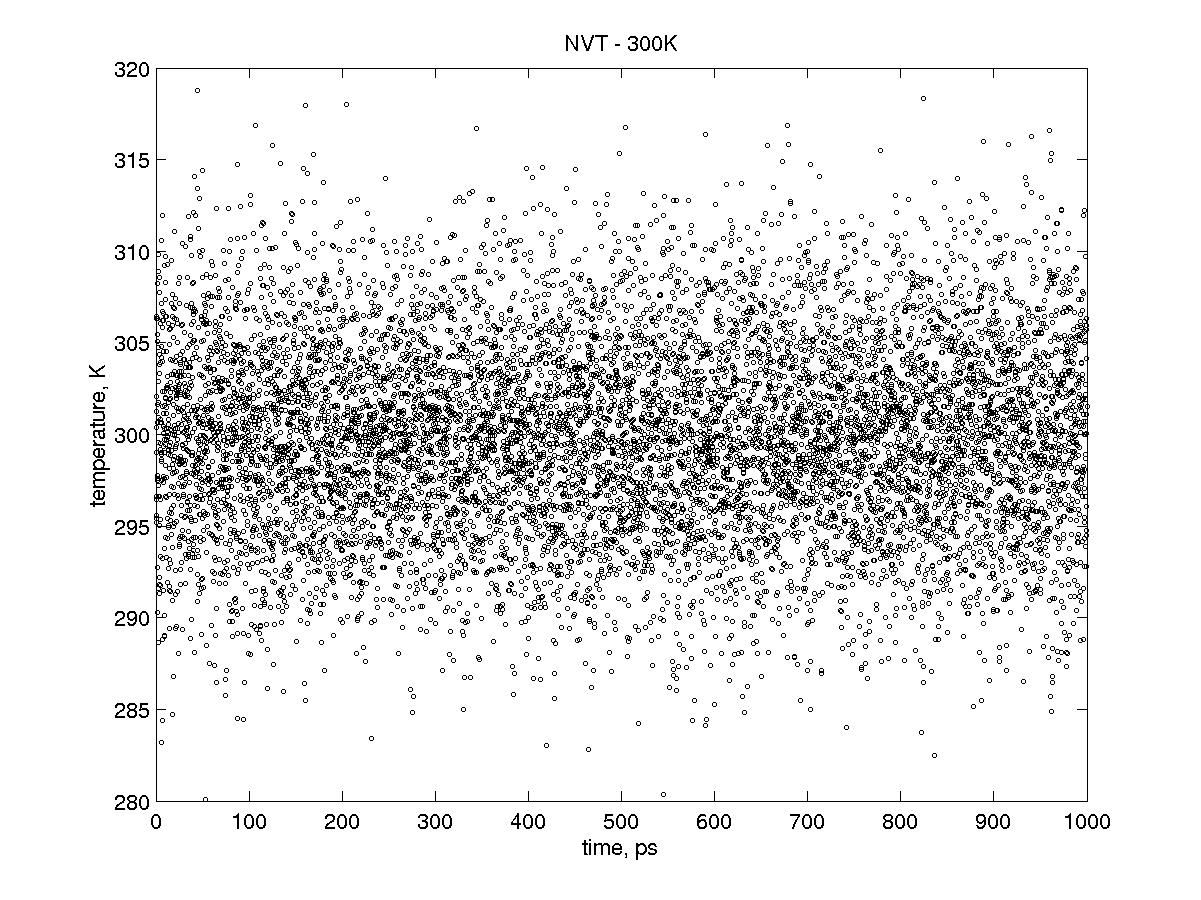
\includegraphics[width=.85\textwidth]{pics/temp_osc2.jpeg}
	\label{fig:temp_osc2}
	\captionof{figure}{Natural temperature fluctuation.}
\end{center}




\section{Stochastic method}

This method, proposed by Andersen \citep{andersen_thermostat}, is a combination of the velocity rescaling and Monte Carlo. At temperature $T$, one expects the velocity distribution to recover the Maxwell-Boltzmann distribution:

\begin{equation}
P\kl{\vec{p}} = \frac{1}{\kl{\pi k T}^\frac{3}{2}} \text{exp}\ekl{ - \frac{\kl{\vec{p}-\vec{p}_0}^2}{kT}  }.
\label{eq:bltz_vert}
\end{equation}

Regularly, every $n$ time steps, the simulation will be suspended and particles are selected randomly and given a new velocity according to \eqref{eq:bltz_vert}. If this is done very often, this method converges towards pure Monte Carlo, if this happens very rarely, the method converges towards classical molecular dynamics. In this hybrid method $n$ becomes an adjustable artificial parameter  that couples the heat bath to the system. The smaller $n$, the larger the coupling to the heat bath is. If the parameter is too large, the system is microcanonical. In a proper simulation, the value of $n$ must be related to the system, e.g. to the number of particles.


\vspace{0.1cm}
\noindent
\begin{minipage}{\textwidth}
\begin{minipage}{.001\textwidth}
 \end{minipage}\hfill
\begin{minipage}{.99\textwidth}
  \centering
  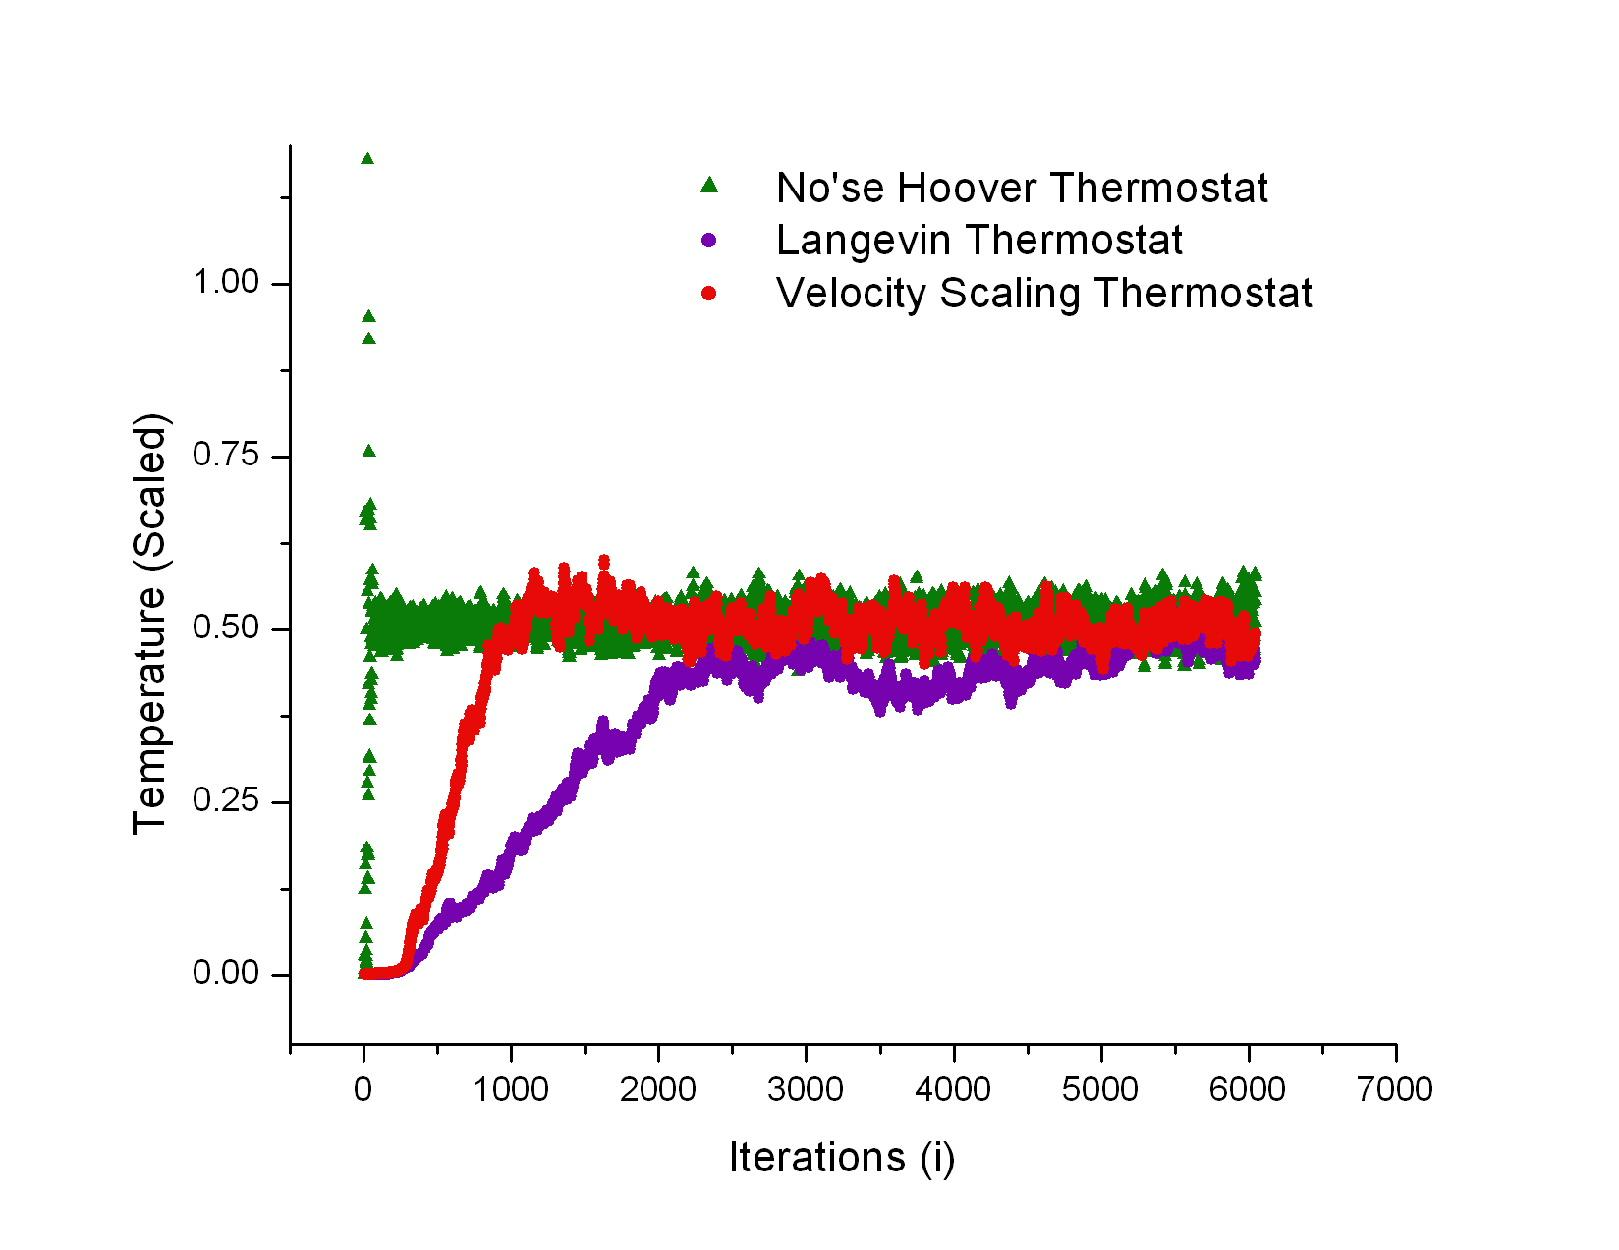
\includegraphics[width=\textwidth]{pics/thermostats.jpg}
  \captionof{figure}{Comparison of the thermostats method and their convergence.}
  \label{fig:thermostats_comp}
\end{minipage}
\end{minipage}
\vspace{0.1cm}




\section{Constant Pressure}

The other classical situation is the one in which pressure is constant. We will again make use of generalized partition theorem \eqref{eq:equipartition} with the Hamiltonian
\begin{equation*}
\mathcal{H} = K\kl{\vec{p}} + V\kl{\vec{x}}
\end{equation*}
Taking the derivative of the hamiltonian with respect to the spatial component yields
\begin{equation*}
\frac{1}{3}\avkl{    \sum^N_{i=1}\vec{x}_i \cdot \kl{ \nabla_{\vec{x}_i} V\kl{\vec{x}}   }    } = NkT.
\end{equation*}
This quantity has the dimension of energy, the prefactor depends on the dimension of the system. We can distinguish inter-particle forces  from those between particles and the volume's surface:
\begin{align*}
&=-\frac{1}{3}\avkl{    \sum^N_{i=1}\vec{x}_i \cdot \kl{ \vec{f}_i^{\text{ext}} + \vec{f}_i^{\text{part}}   }    } \\
&=-\frac{1}{3}\avkl{\sum^N_{i=1}\vec{x}_i \cdot \kl{ \vec{f}_i^{\text{ext}}   }    } 
\underbrace{-\frac{1}{3}\avkl{\sum^N_{i=1}\vec{x}_i \cdot \kl{  \vec{f}_i^{\text{part}}   }    } }_{\equiv\text{virial}}.
\end{align*}

Where \emph{virial} denotes the force that one must apply to keep the system at a certain volume, i.e. the pressure.

\begin{equation*}
\frac{1}{3}\avkl{\sum^N_{i=1}\vec{x}_i \cdot \kl{  \vec{f}_i^{\text{part}}   }    } 
=
-\frac{1}{3} \int_\Gamma p\vec{x} \text{d}\vec{A}
=
-\frac{1}{3} p \int_V \kl{\nabla\cdot\vec{x}} \text{d}\vec{V} 
=
-pV
\end{equation*}

We can thus define the instantaneous pressure as

\begin{equation}
\mathcal{P}  \equiv NkT + \avkl{w}
\label{eq:inst_press}
\end{equation}


For the implementation of a simulation at constant pressure we can use the same method as for the Hoover thermostat. We will introduce a sort of ``pressure bath''. One can imagine this as a piston that changes the volume of the system. Our degree of freedom is a change in volume, hence also in length. As in the Hoover thermostat, we can introduce an artificial parameter 
$W$ that describes how strong the system is coupled to the pressure bath. A useful image is that $W$ corresponds to the weight of the piston: the heavier the piston, the more difficult it is for the system to change a given temperature.

The volume change can be written as: 
\begin{equation}
V = 1- \alpha_T \frac{\Delta}{t_p}\kl{p-\mathcal{P}}
\end{equation} 
where $\alpha_T$ is the isothermal compressibility and $t_p$ is a relaxation time for the pressure. This gives us the factor by which we have to rescale the lentghs $\vec{x}\rightarrow V^\frac{1}{3}\vec{x}$. This is only true in isotropic systems, where a change in length is the same in every directions. In this case, we can just rescale the derivatives as before. The rescaled Hamiltonian is then given by
\begin{equation}
\mathcal{H} = \sum_{i=1}^N \frac{1}{2} m_i \dot{\vec{x}}_i^2  + \frac{1}{2} W\dot{V}^2 + V\kl{ \vec{x}_1,...,\vec{x}_N  } + pV
\end{equation} 
where the new variable V is a volume change controlled by a piston of mass W, that also defines the canonical momentum 
\begin{equation}
p_V= W\dot{V}
\end{equation} 

The equations of motion can be then derived from the Hamiltonian, as usual. The difference from the Hoover thermostat is that the velocities and the kinetic energy do not change while the potential is affected by the spatial rescaling:

$$
\der{\vec{x}_i}{t} = \pder{\mathcal{H}}{\vec{p}_i} = \frac{\vec{p}_i}{m_i V^{\frac{1}{3}}}
$$
$$
\der{V}{t} = \pder{\mathcal{H}}{p_V} = \frac{p_V}{W}
$$
$$
\der{\vec{p}_i}{t} = - \pder{\mathcal{H}}{\vec{x}_i} = -\nabla_{\vec{x}_i} \mathcal{V}\kl{V^{\frac{1}{3}}\vec{x}_i}= \vec{f}_i
$$


$$
\der{p_V}{t} = - \pder{\mathcal{H}}{V} = -\frac{1}{3V}\sum_{i=1}^N\kl{\vec{x}_i\cdot\nabla_{\vec{x}_i} \mathcal{V}\kl{V^{\frac{1}{3}}\vec{x}_i}} -p
$$

In the Berendsen barostat the equations of motion boil down to



\begin{equation}
\ddot{\vec{x}}_i = \frac{\vec{f}_i}{m_i} - \frac{\dot{V}}{3V}\vec{x}_i
\end{equation} 

\begin{equation}
W\ddot{V} = \underbrace{\frac{1}{3V} \sum_{i=1}^N m_i \dot{\vec{x}}_i^2 + \frac{1}{3V} \sum_{i=1}^N \vec{f}_i\vec{x}_i}_{\text{instantaneous pressure }\mathcal{P}} \, - \,p
\end{equation} 



\section{Parrinello-Rahman Barostat}

The problem with the Hoover thermostat is that isotropic space is assumed, as well as a medium like an isotropic gas of molecules. This is generally not the case. In the case of solids (e.g. crystals), the volume cannot be rescaled equally in every direction, since the reaction to pressure and pressure changes can be different along different directions. The first and simplest generalization is an orthogonal scaling of a box described by three vectors, $\vec{a}, \vec{b}$ and $\vec{c}$ of a volume


\begin{equation}
V= \vec{a}\cdot \kl{\vec{b}\times\vec{c}} = \text{det}\kl{\mat{H}}\hspace{0.4cm}\text{with }\mat{H} = \mkl{\vec{a},\vec{b},\vec{c}}.
\end{equation}


The position of a particle $i$ in the box can then be described by
\begin{equation}
\vec{r}_i = \mat{H} \vec{s}_i = x_i \vec{a} + y_i \vec{b} + z_i \vec{c} \hspace{0.4cm}\text{with }0<x_i,y_i,z_i<1.
\end{equation}
From this definition follows the distance between two particles $i$ and $j$:


\begin{equation}
\vec{r}_{i,j}^{\,2} =\vec{s}_{i,j}^{\,T} \mat{G} \vec{s}_{i,j}  \hspace{0.4cm}\text{with }\mat{G} = \mat{H}^{\,T}\, \mat{H}
\end{equation}

The Hamiltonian can then be then expressed using the new distances:

\begin{equation}
\mathcal{H} = \frac{1}{2} \sum_i m_i\dot{\vec{s}}_{i}^{\,T} \mat{G} \dot{\vec{s}}_{i} +  \sum_{i,j} \mathcal{V}\kl{\vec{r}_{i,j}} + \frac{1}{2} W \text{Tr}\kl { \dot{ \mat{H}} ^{\,T} \dot{\mat{H}}  } + pV
\end{equation}

Again, one can derive the equations of motion from the Hamiltonian in the usual way and the result,

\begin{equation}
m_i\ddot{\vec{s}}_i = \mat{H}^{-1} \vec{f}_i - m_i \mat{G}^{-1}\kl{\dot{\mat{G}}\dot{\vec{s}}_i}
\end{equation}

\begin{equation}
W\ddot{\mat{H}} = \mat{p} V \kl{\mat{H}^{-1}}^T
\end{equation}
is very important when simulating crystals, e.g. in solid state physics or in material science. Our degree of freedom is not a simple scalar like in the Hoover thermostat, but it is a tensor ($\mat{H}$) given by the geometry of the system. In the case of constant pressure and temperature, one can use a combination of the two: the $NpT$ ensemble (also known as isothermal-isobaric ensemble) which we will not treat here.










% \subsection{Fluid Dynamics} ?
% \subsection{Lattice} ?
% \subsection{quantum mechanics} ?

















